\documentclass[a4paper]{article}
\usepackage[pdftex]{graphicx}
\usepackage[utf8]{inputenc}
\usepackage{enumerate}
\usepackage{siunitx}
\sisetup{locale=DE} 
\usepackage{href-ul}
\hypersetup{
	colorlinks=true,
	linkcolor=blue,
	urlcolor=blue}
\usepackage{icomma} 
\usepackage{colortbl}
\usepackage{multirow}
\usepackage{amssymb}
\usepackage{tikz}
\usetikzlibrary{positioning}
\usepackage{geometry}
\geometry{a4paper, top=15mm, left=15mm, right=15mm, bottom=15mm,
	headsep=10mm, footskip=12mm}

%Source: img_0243

% Start the document
\begin{document}
%Titel
{\bf Parallel- und Reihenschaltung von Widerständen }\\
\begin{minipage}{0.5\textwidth}

%Aufgabe 1
Du hast folgende Widerstände:\\ 2 x \fbox{$R=\SI{10}{\ohm}$}\\
2 x \fbox{$R=\SI{33}{\ohm}$}\\
2 x \fbox{$R=\SI{100}{\ohm}$}\\


\end{minipage}
\hfill
\begin{minipage}{0.5\textwidth}

	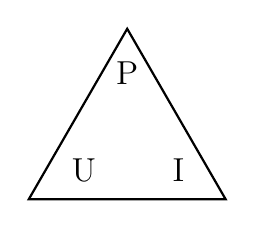
\begin{tikzpicture}[scale=1]
	% Dreieck mit Seitenlänge 2.5 cm
	\coordinate (U) at (0,0);
	\coordinate (I) at (2.5,0);
	\coordinate (P) at (1.25, {2.5*sqrt(3)/2});
	
	% Linien zeichnen
	\draw[thick] (U) -- (I) -- (P) -- cycle;
	
	% Beschriftung innerhalb
	\node[above=0.1cm of U, xshift=0.7cm] {\large U};
	\node[above=0.1cm of I, xshift=-0.6cm] {\large I};
	\node[below=0.3cm of P] {\large P};
\end{tikzpicture}
\hspace{3 cm}
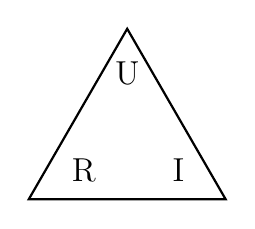
\begin{tikzpicture}[scale=1]
	% Dreieck mit Seitenlänge 2.5 cm
	\coordinate (R) at (0,0);
	\coordinate (I) at (2.5,0);
	\coordinate (U) at (1.25, {2.5*sqrt(3)/2});
	
	% Linien zeichnen
	\draw[thick] (R) -- (I) -- (U) -- cycle;
	
	% Beschriftung innerhalb
	\node[above=0.1cm of R, xshift=0.7cm] {\large R};
	\node[above=0.1cm of I, xshift=-0.6cm] {\large I};
	\node[below=0.3cm of U] {\large U};
\end{tikzpicture}
\end{minipage}

\begin{enumerate}[1.]
	{\bf \item Schließe jeden Widerstand an eine Stromquelle 5V} an und ermittle die Stromstärke und die Leistung. Welcher Widerstand hat die höchste Leistung?
	
	{\bf Trage die berechneten und gemessenen Widerstandswerte in die Tabelle ein.}
	
\begin{minipage}{0.5\textwidth}
	\item  Reihenschaltung 
	
	\renewcommand{\arraystretch}{2}
	\begin{tabular}{|>{\columncolor[gray]{.8}}p{1.5 cm}|p{1.5 cm}|p{1.5 cm}|p{1.5 cm}|}
		\hline
		\rowcolor[gray]{.8}	 $R_1 +R_2$ & $\SI{10}{\ohm}$	& $\SI{33}{\ohm}$	& $\SI{100}{\ohm}$	\\
		\hline
		\multirow{2}{*}{\vspace*{0.2cm}$\SI{10}{\ohm}$} 	& & & \\ \cline{2-4}
		& & & \\
		\hline
		\multirow{2}{*}{\vspace*{0.2cm}$\SI{33}{\ohm}$} 	& & & \\ \cline{2-4}
		& & & \\
		\hline
		\multirow{2}{*}{\vspace*{0.2cm}$\SI{100}{\ohm}$} 	& & & \\ \cline{2-4}
		& & & \\
		\hline
	\end{tabular}
\end{minipage}
\hfill
\begin{minipage}{0.5\textwidth}
	\item Parallelschaltung
	
	\renewcommand{\arraystretch}{2}
	\begin{tabular}{|>{\columncolor[gray]{.8}}p{2 cm}|p{1.5 cm}|p{1.5 cm}|p{1.5 cm}|}
		\hline
		\rowcolor[gray]{.8}	 $\left(\frac{1}{R_1}+\frac{1}{R_2}\right)^{-1}$ & $\SI{10}{\ohm}$	& $\SI{33}{\ohm}$	& $\SI{100}{\ohm}$	\\
		\hline
		\multirow{2}{*}{\vspace*{0.2cm}$\SI{10}{\ohm}$} 	& & & \\ \cline{2-4}
		& & & \\
		\hline
		\multirow{2}{*}{\vspace*{0.2cm}$\SI{33}{\ohm}$} 	& & & \\ \cline{2-4}
		& & & \\
		\hline
		\multirow{2}{*}{\vspace*{0.2cm}$\SI{100}{\ohm}$} 	& & & \\ \cline{2-4}
		& & & \\
		\hline
	\end{tabular}
\end{minipage}	
{\bf \item Welche Widerstände schaltest Du, um einen möglichst ...}\\

\begin{enumerate}[a)]

\hspace{-2 cm}
\begin{minipage}{0.3\textwidth}
\includegraphics[width=5 cm]{1wisch243.pdf}
\end{minipage}
\hspace{-0.5cm}
\begin{minipage}{0.3\textwidth}
 \item ...großen Gesamtwiderstand zu erhalten?\\
 
 	\renewcommand{\arraystretch}{2}
	\begin{tabular}{|>{\columncolor[gray]{.8}}p{1cm}|p{0.8cm}|p{0.8cm}|p{0.8cm}|p{0.8cm}|}
	\hline
	\rowcolor[gray]{.8}	  & $R$ & $U$	& $I$	 & $P$\\
	\hline
 1 & & &  & \\
 	\hline
 2	& & &  & \\
 	\hline
 3 & & &  & \\
 	\hline
 Gesamt & & $\SI{5,0}{\volt}$&  & \\
	\hline
\end{tabular}
\end{minipage}
\hspace{1cm}
\begin{minipage}{0.3\textwidth}
\item ...kleinen Gesamtwiderstand zu erhalten?\\

	\renewcommand{\arraystretch}{2}
	\begin{tabular}{|>{\columncolor[gray]{.8}}p{1cm}|p{0.8cm}|p{0.8cm}|p{0.8cm}|p{0.8cm}|}
	\hline
	\rowcolor[gray]{.8}	  & $R$ & $U$	& $I$	 & $P$ \\
	\hline
	1 & & &  & \\
	\hline
	2	& & &  & \\
	\hline
	3 & & &  & \\
	\hline
	Gesamt & & $\SI{5,0}{\volt}$&  & \\
	\hline
\end{tabular}
\end{minipage}

\hspace{-2 cm}
\begin{minipage}{0.3\textwidth}
	\includegraphics[width=5 cm]{2wisch243.pdf}
\end{minipage}
\hspace{-0.5cm}
\begin{minipage}{0.3\textwidth}
	\item ...großen Gesamtwiderstand zu erhalten?\\
	
		\renewcommand{\arraystretch}{2}
	\begin{tabular}{|>{\columncolor[gray]{.8}}p{1cm}|p{0.8cm}|p{0.8cm}|p{0.8cm}|p{0.8cm}|}
		\hline
		\rowcolor[gray]{.8}	  & $R$ & $U$	& $I$	 & $P$ \\
		\hline
		1 & & &  & \\
		\hline
		2	& & &  & \\
		\hline
		3 & & &  & \\
		\hline
		Gesamt & & $\SI{5,0}{\volt}$&  & \\
		\hline
	\end{tabular}
\end{minipage}
\hspace{1cm}
\begin{minipage}{0.3\textwidth}
	\item ...kleinen Gesamtwiderstand zu erhalten?\\
	
		\renewcommand{\arraystretch}{2}
	\begin{tabular}{|>{\columncolor[gray]{.8}}p{1cm}|p{0.8cm}|p{0.8cm}|p{0.8cm}|p{0.8cm}|}
		\hline
		\rowcolor[gray]{.8}	  & $R$ & $U$	& $I$	 & $P$\\
		\hline
		1 & & &  & \\
		\hline
		2	& & &  & \\
		\hline
		3 & & &  & \\
		\hline
		Gesamt & & $\SI{5,0}{\volt}$&  & \\
		\hline
	\end{tabular}
\end{minipage}


\end{enumerate}


\end{enumerate} 

\fbox{
	\begin{minipage}{0.5\textwidth}
		Zur Lösung bitte \href{https://www.okuyakl.de/phys/p8wipareiL243/ll243.pdf}{hier klicken} oder den QR-Code scannen.\\
	Weitere Arbeitsblätter gibt es unter 
	
	\href{https://www.okuyakl.de}{www.okuyakl.de}
	\end{minipage}
	\hfill
	\begin{minipage}{0.4\textwidth}
		\includegraphics[width=1.5 cm]{../../viecher/zwe03}
		\includegraphics[width=3 cm]{qr243}
		\includegraphics[width=2 cm]{../../viecher/afanticon1}
		
	\end{minipage}}
\end{document}
